\subsection*{Question 1}


$0,75=\dfrac{3}{4}$, mais aussi \mbox{$\np{0.75}=\dfrac{75}{100}$}, il n'est pas demandé que la fraction soit irréductible.

\subsection*{Question 2}

$-4,7+3,5=-(1,2+3,5)+3,5=-1,2-3,5+3,5=-1,2$.
\subsection*{Question 3}


$a=\dfrac{12\times 18}{6}=\dfrac{12}{6}\times 18=2\times 18 =36$.

\textit{Variante (1)} : c'est un tableau de proportionnalité et dans la première colonne 12 est le double de 6, donc $a$ est le double de 18 c'est-à-dire 36.

\textit{Variante (2)} : puisque c'est un tableau de proportionnalité et que dans la ligne du haut 18 est le triple de 6, alors $a$ est le triple de 12 donc 36.
\subsection*{Question 4}


$10+4=6=20$.

Il y a 20 boules, dont 4 sont bleues.

La probabilité de tirer une bleue est donc de $\dfrac{4}{20}$,  \textbf{réponse B}.

\subsection*{Question 5}

\begin{align*}
10 x+16&=-64\\
10x&=-64-16\\
10x &=-80\\
x&=\dfrac{-80}{10}\\
x&=-8
\end{align*}
 Donc \textbf{réponse C : $-8$}.

\subsection*{Question 6}

$\np{0,00458}=4,58\times 10^{-3}$.

Donc \textbf{réponse C}

\subsection*{Question 7}


On remarque que l'angle pour la section de la réponse B est un angle droit. Il correspond donc à un quart de 360°.

$\dfrac{1}{4}\times 24=6$.

Donc six élèves ont choisi la réponse B.

\subsection*{Question 8}

$10\times 2 +5\times 2=30$ mm.

Donc \textbf{réponse A}.

\subsection*{Question 9}

\begin{minipage}[t]{0.45\linewidth}\vspace{0mm}
	\begin{align*}
\cos(\widehat{\text{EDF}})&=\dfrac{\text{adjacent}}{\text{hypoténuse}}\\
\cos(\widehat{\text{EDF}})&=\dfrac{\text{DE}}{\text{DF}}\\
&=\dfrac{6}{10}\\
&=\dfrac{3}{5}
\end{align*}

\end{minipage}\hspace{0.05\linewidth}\begin{minipage}[t]{0.45\linewidth}\vspace{0mm}
\begin{adjustbox}{max width=1\linewidth,max totalheight=255mm}
	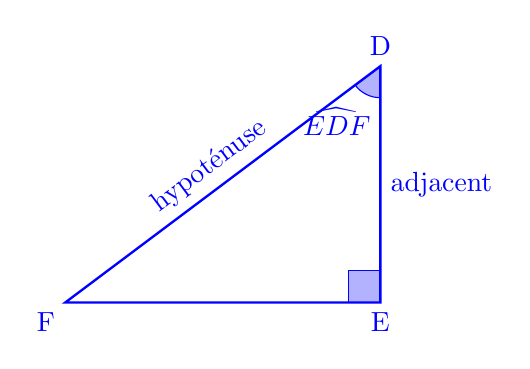
\begin{tikzpicture}[xscale=1,yscale=1,rotate=0,every node/.style={scale=1,rotate=0}]
		\draw[blue, fill=blue!30](4,3)--(4,2.6)node[below left]{$\widehat{\text{EDF}}$}arc(-90:-143.13:0.4)--cycle;
		\draw[blue, fill=blue!30](3.6,0.4)rectangle(4,0);
		\draw[blue, line width=0.3mm](4,0)node[below]{E}--(4,3)node[above]{D}node[midway, right]{adjacent}--(0,0)node[below left]{F}node[midway, above,sloped]{hypoténuse}--cycle;
	\end{tikzpicture}
\end{adjustbox}
\end{minipage}


Donc  \textbf{réponse B}



\vspace{10mm}
\needspace{10\baselineskip}

% saut de page si moins de 10 lignes disponibles
